% ======================================================================
\section{SGD with momentum}\label{sec:momentum}
% ======================================================================

\subsection{The algorithm and its equivalent forms}\label{sec:forms}

\begin{tcolorbox}[keybox,title={\textbf{Algorithm 1: SGD with momentum (heavy-ball form)}},
  colbacktitle=RoyalBlue!60!black]
\textbf{Input:} starting point $x_0\in\R^d$, step size $\alpha>0$, momentum $\beta\in[0,1)$.
Set $x_{-1}:=x_0$.\\
\textbf{For} $k=0,1,2,\dots$:
\begin{enumerate}[label=\arabic*.,leftmargin=2.2em,topsep=2pt]
  \item draw a fresh sample $\xi_k$ and compute $g_k=g(x_k;\xi_k)$;
  \item update $x_{k+1}=x_k-\alpha\,g_k+\beta\,(x_k-x_{k-1})$.
\end{enumerate}
\end{tcolorbox}

Software libraries usually implement momentum through an auxiliary ``buffer''. The next
proposition shows that the common variants are the same algorithm.

\begin{proposition}[Three equivalent forms]\label{prop:forms}
Run the following three recursions with the same samples $\xi_0,\xi_1,\dots$, the same
$x_0$, and $\gamma:=\alpha/(1-\beta)$:
\begin{enumerate}[label=\textup{(\roman*)}]
\item \emph{heavy-ball form:} $x_{k+1}=x_k-\alpha g_k+\beta(x_k-x_{k-1})$, \quad $x_{-1}=x_0$;
\item \emph{momentum-buffer form:} $m_k=\beta m_{k-1}+g_k$, \quad $x_{k+1}=x_k-\alpha m_k$,
      \quad $m_{-1}=0$;
\item \emph{averaging form:} $\bar m_k=\beta\bar m_{k-1}+(1-\beta)g_k$, \quad
      $x_{k+1}=x_k-\gamma\bar m_k$, \quad $\bar m_{-1}=0$.
\end{enumerate}
They produce identical iterates $x_0,x_1,x_2,\dots$ Moreover
$m_k=\sum_{j=0}^k\beta^{k-j}g_j$ and $\bar m_k=(1-\beta)m_k$.
\end{proposition}

\begin{proof}
Unrolling (ii) by induction gives $m_k=g_k+\beta m_{k-1}=\sum_{j=0}^k\beta^{k-j}g_j$.
Next, the iterates of (ii) satisfy the recursion (i): for $k\ge1$,
\[
  x_{k+1}-x_k=-\alpha m_k=-\alpha(\beta m_{k-1}+g_k)=\beta(-\alpha m_{k-1})-\alpha g_k
  =\beta(x_k-x_{k-1})-\alpha g_k,
\]
and for $k=0$, $x_1-x_0=-\alpha m_0=-\alpha g_0=\beta(x_0-x_{-1})-\alpha g_0$ because
$x_{-1}=x_0$. Both recursions start at $x_0$; if their iterates agree up to index $k$, then
$g_k=g(x_k;\xi_k)$ agrees too, and so does $x_{k+1}$. By induction the iterates coincide.
For (iii), $\bar m_k=(1-\beta)m_k$ holds for $k=-1$ and is preserved by the recursions
(multiply the recursion for $m_k$ by $1-\beta$); hence $\gamma\bar m_k=\gamma(1-\beta)m_k=\alpha m_k$.
\end{proof}

Form (ii) is, for instance, PyTorch's momentum SGD, with learning rate $\alpha$. Form (iii)
is the ``exponential moving average'' form (used, e.g., for the first moment in Adam);
there the learning rate \emph{is} the effective step size $\gamma$ introduced next. When
comparing papers or code, always check which form is meant: the same symbol ``learning
rate'' can mean $\alpha$ or $\gamma=\alpha/(1-\beta)$, a factor of $10$ apart when $\beta=0.9$.

\subsection{The effective step size}\label{sec:effective}

By \cref{prop:forms}, the displacement at step $k$ is $-\alpha m_k=-\alpha\sum_{j\le k}\beta^{k-j}g_j$,
an exponentially weighted sum of all past stochastic gradients. If the gradients were all
equal to some vector $g$, this would be
\[
  -\alpha\,\frac{1-\beta^{k+1}}{1-\beta}\,g\;\longrightarrow\;-\frac{\alpha}{1-\beta}\,g=-\gamma\,g .
\]
So in a region where the gradient changes slowly, SGDM moves like SGD with step size
\begin{equation}\label{eq:gamma}
  \gamma:=\frac{\alpha}{1-\beta}\qquad(\text{effective step size}).
\end{equation}
With $\beta=0.9$, $\gamma=10\alpha$. The effective step size will appear in every result
below, and it is the right quantity for comparing SGDM with SGD (\cref{sec:experiments}).

\subsection{Why the function value is the wrong yardstick}\label{sec:naive}

Let us try to copy the proof of \cref{lem:sgd-step}. Define the \emph{velocity}
\begin{equation}\label{eq:velocity}
  v_k:=x_k-x_{k-1}\quad(k\ge0),\qquad v_0=0,\qquad\text{so that}\qquad
  v_{k+1}=\beta v_k-\alpha g_k .
\end{equation}
The descent lemma with $x=x_k$, $y=x_{k+1}=x_k+v_{k+1}$ gives
$f(x_{k+1})\le f(x_k)+\ip{\nabla f(x_k)}{\beta v_k-\alpha g_k}+\frac L2\norm{\beta v_k-\alpha g_k}^2$.
Since $v_k$ is known at time $k$, taking $\Ek$ yields
\begin{equation}\label{eq:naive}
  \Ek[f(x_{k+1})]\le f(x_k)-\alpha\norm{\nabla f(x_k)}^2
  +\underbrace{\beta\ip{\nabla f(x_k)}{v_k}}_{\text{inertia term}}
  +\frac L2\,\Ek\norm{\beta v_k-\alpha g_k}^2 .
\end{equation}
Compared with \cref{lem:sgd-step} there is a new \emph{inertia term}. It is a problem for
two reasons. First, it is linear in the velocity, and the velocity is itself of the order
of the step size ($v_k=-\alpha m_{k-1}$), so the inertia term is of the \emph{same order}
as the progress term $-\alpha\norm{\nabla f(x_k)}^2$; making $\alpha$ small does not make
it negligible. Second, its sign is arbitrary: after the ball overshoots the bottom of a
valley, the last step $v_k$ points uphill at $x_k$ and the term is positive. The following
example shows that this really happens.

\begin{example}[Momentum pushes the iterate away from the minimizer]\label{ex:overshoot}
Let $f(x)=\frac12x^2$ on $\R$ (so $L=1$, $x^\star=0$, $\fs=0$), use exact gradients
($g_k=x_k$), $\alpha=1$, $\beta=\frac12$, and $x_{-1}=x_0=1$. The update becomes
$x_{k+1}=x_k-x_k+\frac12(x_k-x_{k-1})=\frac12(x_k-x_{k-1})$, and the iterates are
\begin{center}
\renewcommand{\arraystretch}{1.35}
\begin{tabular}{@{}c|cccccccc@{}}
$k$ & $0$ & $1$ & $2$ & $3$ & $4$ & $5$ & $6$ & $7$\\\hline
$x_k$ & $1$ & $0$ & $-\frac12$ & $-\frac14$ & $\frac18$ & $\frac3{16}$ & $\frac1{32}$ & $-\frac5{64}$\\
$f(x_k)$ & $\frac12$ & $0$ & $\frac18$ & $\frac1{32}$ & $\frac1{128}$ & $\frac9{512}$ & $\frac1{2048}$ & $\frac{25}{8192}$
\end{tabular}
\end{center}
At $k=1$ the iterate sits \emph{exactly at the minimizer}, with zero gradient. Nevertheless
its velocity $v_1=-1$ carries it away: $f(x_2)=\frac18>0=f(x_1)$. The function value goes
up again from $k=4$ to $k=5$ and from $k=6$ to $k=7$. (The method still converges here, see
\cref{prop:quadratic-stability}.) \Cref{fig:potential}(b) shows the same non-monotone
behaviour for $\beta=0.9$ and a step size small enough for all our theorems to apply.
\end{example}

So no inequality of the form \eqref{eq:intro-sgd-decrease} can hold for SGDM in general.
What \emph{can} be said about one step, measured by $f$ itself, is the following.

\begin{proposition}[One SGDM step measured by $f$]\label{prop:f-step}
Under \cref{as:smooth,as:unbiased,as:variance}, for every $k\ge0$,
\begin{equation}\label{eq:f-step}
  \Ek[f(x_{k+1})]\le f(x_k)-\alpha(1-L\alpha)\norm{\nabla f(x_k)}^2
  +\beta\ip{\nabla f(x_k)}{v_k}+L\beta^2\norm{v_k}^2+\frac{L\alpha^2}{2}\sigma^2 .
\end{equation}
Consequently, if $\alpha\le\frac1{2L}$ and the last step points sufficiently downhill,
\begin{equation}\label{eq:downhill}
  \ip{\nabla f(x_k)}{v_k}\le-L\beta\norm{v_k}^2,
\end{equation}
then $\Ek[f(x_{k+1})]\le f(x_k)-\frac\alpha2\norm{\nabla f(x_k)}^2+\frac{L\alpha^2}{2}\sigma^2$:
exactly the SGD inequality of \cref{lem:sgd-step}.
\end{proposition}

\begin{proof}
By the variance decomposition (\cref{lem:variance}; the conditional mean of
$\beta v_k-\alpha g_k$ is $\beta v_k-\alpha\nabla f(x_k)$) and \cref{lem:elementary}(e),
\[
  \Ek\norm{\beta v_k-\alpha g_k}^2=\norm{\beta v_k-\alpha\nabla f(x_k)}^2+\alpha^2\Ek\norm{\eps_k}^2
  \le2\beta^2\norm{v_k}^2+2\alpha^2\norm{\nabla f(x_k)}^2+\alpha^2\sigma^2 .
\]
Multiply by $\frac L2$ and insert into \eqref{eq:naive}; this gives \eqref{eq:f-step}. Under
\eqref{eq:downhill}, $\beta\ip{\nabla f(x_k)}{v_k}+L\beta^2\norm{v_k}^2\le0$, and
$1-L\alpha\ge\frac12$ when $\alpha\le\frac1{2L}$.
\end{proof}

So the function value decreases in expectation just as for SGD as long as the momentum
still points downhill; after an overshoot, when $\ip{\nabla f(x_k)}{v_k}>0$, no decrease can
be guaranteed. The algorithm has no control over the sign of this inner product, so a
guarantee that holds at \emph{every} step needs a different quantity to measure progress.

\subsection{The extrapolated point}\label{sec:extrapolated}

\begin{definition}[Extrapolated point]
For $k\ge0$ let
\begin{equation}\label{eq:z}
  z_k:=x_k+\frac{\beta}{1-\beta}\,v_k=x_k+\frac{\beta}{1-\beta}\,(x_k-x_{k-1}).
\end{equation}
\end{definition}

\begin{lemma}[The extrapolated points perform SGD]\label{lem:z}
For SGDM (Algorithm~1), $z_0=x_0$ and, for every $k\ge0$,
\begin{equation}\label{eq:z-sgd}
  z_{k+1}=z_k-\gamma\,g_k,\qquad\gamma=\frac{\alpha}{1-\beta}.
\end{equation}
\end{lemma}

\begin{proof}
$z_0=x_0$ because $v_0=0$. Using $x_{k+1}-x_k=v_{k+1}$ and the velocity recursion
$v_{k+1}=\beta v_k-\alpha g_k$ from \eqref{eq:velocity},
\[
  z_{k+1}-z_k=v_{k+1}+\frac{\beta}{1-\beta}(v_{k+1}-v_k)
  =\frac{1}{1-\beta}\bigl(v_{k+1}-\beta v_k\bigr)=\frac{-\alpha g_k}{1-\beta}=-\gamma g_k .\qedhere
\]
\end{proof}

\begin{tcolorbox}[intuition,title=Physical meaning of $z_k$]
Suppose that from time $k$ on the force is switched off (all gradients are zero). Then
the velocity decays geometrically, $v_{k+j}=\beta^jv_k$, and the ball comes to rest at
\[
  x_k+(\beta+\beta^2+\beta^3+\cdots)\,v_k=x_k+\frac{\beta}{1-\beta}\,v_k=z_k .
\]
So $z_k$ is the \emph{coasting endpoint}: where the ball would stop under friction alone.
A gradient kick $-\alpha g_k$ changes the velocity, and friction carries this change
forward with total amplification $1+\beta+\beta^2+\cdots=\frac1{1-\beta}$. Hence the
coasting endpoint moves by exactly $-\gamma g_k$: \emph{the points $z_k$ perform plain
SGD with step size $\gamma$}---except that the gradient is evaluated at $x_k$ rather than
at $z_k$. The mismatch is controlled by the distance
\begin{equation}\label{eq:z-minus-x}
  \norm{z_k-x_k}=\frac{\beta}{1-\beta}\,\norm{v_k},
\end{equation}
which is proportional to the velocity. \Cref{fig:potential}(a) shows $x_k$ and $z_k$ for
a one-dimensional quadratic: $z_k$ ``looks ahead'' of $x_k$.
\end{tcolorbox}

\begin{remark}[Varying step sizes]\label{rem:varying}
If Algorithm~1 uses a step size $\alpha_k$ at iteration $k$ (heavy-ball form, constant
$\beta$), then $v_{k+1}=\beta v_k-\alpha_kg_k$, and the same computation gives
$z_{k+1}=z_k-\gamma_kg_k$ with $\gamma_k=\alpha_k/(1-\beta)$. (In the momentum-buffer form
a changing $\alpha_k$ rescales the whole buffer, the forms are no longer equivalent, and
this identity fails; we only treat varying steps in heavy-ball form.)
\end{remark}

\begin{figure}[t]
\centering
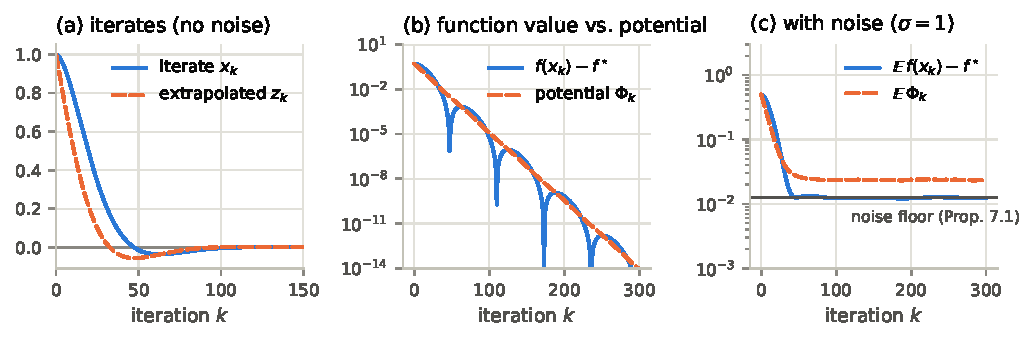
\includegraphics[width=\textwidth]{figures/potential.pdf}
\caption{Heavy ball on $f(x)=\frac12x^2$ ($L=1$) with $\beta=0.9$ and
$\alpha=(1-\beta)^2/(2L)=0.005$, the largest step allowed by \cref{thm:master}(b).
(a)~Without noise: the iterate $x_k$ and the extrapolated point $z_k$, which moves ahead
of $x_k$. (b)~Without noise: $f(x_k)-\fs$ is not monotone (it rises after each
overshoot), while the potential $\Phi_k$ of \cref{thm:master} decreases at every step.
(c)~With noise ($\sigma=1$, average over $20\,000$ runs): both expectations settle at a
noise floor; the floor of $\E f(x_k)$ agrees with the exact value of
\cref{prop:noise-floor} (horizontal line).}
\label{fig:potential}
\end{figure}
